\documentclass[11pt,a4j,fleqn]{jarticle}
\usepackage{amsmath,amsthm,amssymb}
\usepackage[dvipdfmx]{graphicx}

\title{包絡線定理・レポート}
\author{山岸 敦}
\date{2014/6/7}


\begin{document}

\maketitle

\section{はじめに}

(例えば価格のような)パラメーターを含む関数fについての最適化を考えよう。このとき、そのパラメーターに対して最適化された変数をもとの代入するとパラメーターだけを変数とする関数(価値関数と呼ぶ)ができる。fとこの関数の関係として包絡線定理(envelope theorem)があり、これは経済学の様々な分野で応用されている…のだが、このような言葉の説明だけ読んだところで実感できないだろう。ここでは、pythonによって描かれた包絡線定理のグラフをもちいつつ包絡線定理を解説し、その後で描画に用いたpythonプログラムについて解説する。


\section{包絡線定理}

さて、いきなり抽象的な関数に対しての議論は難しいかもしれないのでここでは関数形を特定しよう。

変数tとパラメーターxを持つ関数f
\[
f(x, t) =2 t x - t^2
\]

を想定しよう。

これを、変数tの二次式と見て平方完成すれば
\begin{equation}
f(x, t)  = -(t - x)^2 + x^2 \label{eq:square-1}
\end{equation}

を得る。この関数は$t=x$で最大値$x^2$をとることが(1)の式の形から容易にわかるであろう。この最大値をxの関数とみなし、$V(x)=x^2$ともとの$f(x,t)$の関係を考えよう。

$f(x,t)$の値は、その最大値を取った$V(x)$の値を上回ることはない。t=xの時だけ$V(x)$と$f(x,t)$は同じ値をとり、それ以外の時は$f(x,t)$が下回る。
ここで$f(x,t)$はxについて1次関数なので、以上の条件を考えると、xを横軸にとってプロットすれば$f(x,y)$は$V(x)$に$x=t$の点で接する接線になる。

具体例を出そう。たとえば、$t=2$なら

\begin{equation}
f(x, t) = 2×2x-2^2 = 4x-4
\end{equation}

となるが、これは確かに$x^2$の$x=2$における接線になっている。
この規則(tの値がなんであれ、関数fは常に$x=t$で$x^2$の接線になる)を頭に入れておけば、$f(x,t)$はtの値をどういじっても決して$x^2$を通らないことがわかる。
このことを図を用いて解説しよう。

図1は、tの値を変えて$f(x,t)$を横軸にxを取った平面にプロットしたものである。なんとなく、$x^2$のあたりを通過していないことがわかるだろう。
図2はより多くのtの値に対して$f(x,t)$を同様にプロットしたもので、本数を増やすにつれ$x^2$が浮かび上がってくるのがわかるだろう。
このように、$f(x,t)$の変数tの値を変えたグラフを何本も描くことで、最適値がどうパラメーターによって変わるかを示すグラフ$V(x)$が描ける、というのが包絡線定理の主張である。

\begin{figure}[!p]
\begin{center}
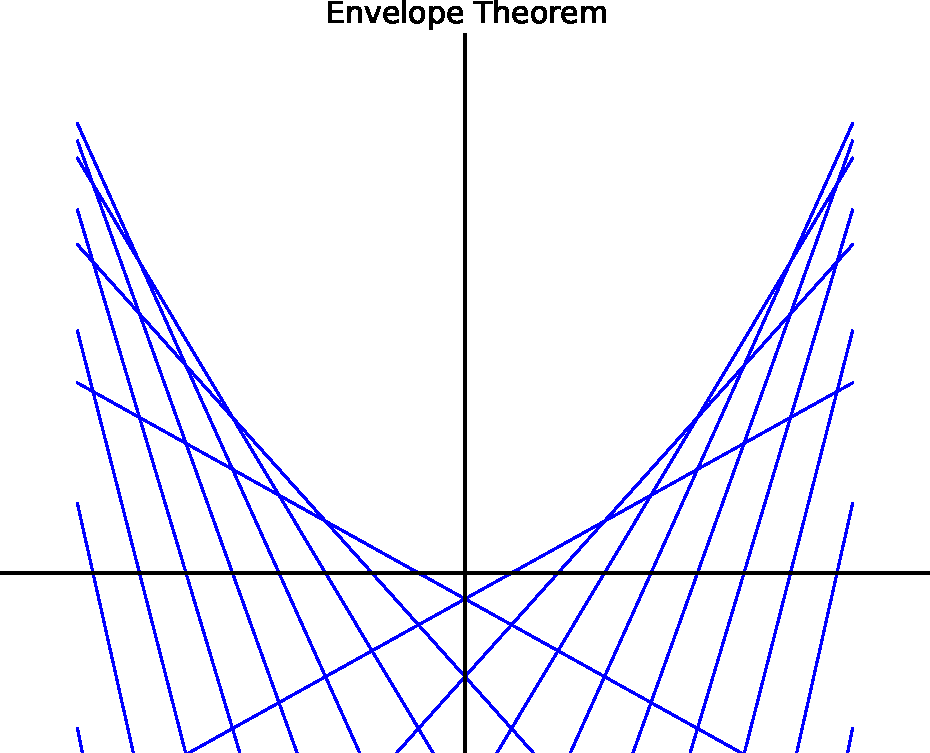
\includegraphics[scale=0.6]{envelope1.pdf}
\end{center}
\caption{接線の本数が少なめの状態}
\label{fig:1}
\end{figure}

\begin{figure}
\begin{center}
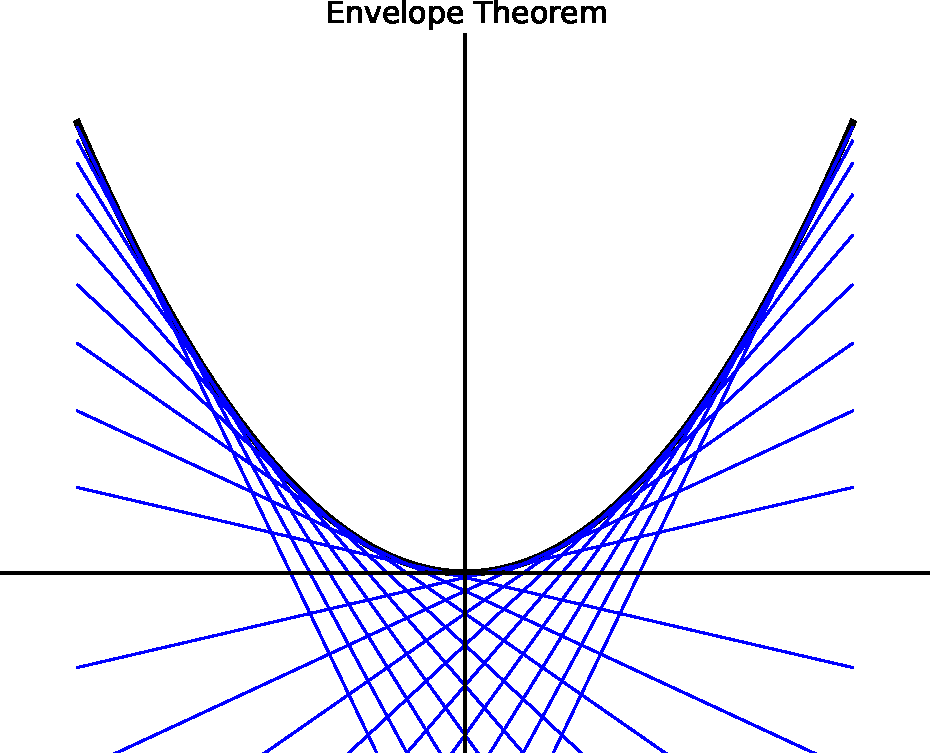
\includegraphics[scale=0.6]{envelope0.pdf}
\end{center}
\caption{多くの接線を引いた状態}
\label{fig:2}
\end{figure}





\section{Pythonプログラム}

自分のPythonプログラムの説明を書く.

コードの表示の例
\begin{quote}
\begin{verbatim}
import numpy
from matplotlib import pyplot
x = numpy.arange(0, 10, 0.1)
y = numpy.cos(x)
pyplot.plot(x,y)
pyplot.show()
\end{verbatim}
\end{quote}

\verb|\begin{verbatim}| ... \verb|\end{verbatim}| の中では改行は自動ではされない.
長すぎてページからはみ出す行は自分で適宜改行する.



\begin{thebibliography}{0}
\bibitem{OyamaYasuda11}
尾山大輔・安田洋祐「経済学で出る包絡線定理」『経済セミナー』2011年10・11月号.
\end{thebibliography}

\end{document}